\documentclass[12pt]{article}
 
\usepackage[margin=1in]{geometry} 
\usepackage{amsmath,amsthm,amssymb,mathtools}
\usepackage{listings}
\usepackage{epstopdf}
\usepackage{soul}
\usepackage{tcolorbox}
\usepackage{indentfirst}
\usepackage{fancyhdr,graphicx,float}
\graphicspath{{figures/}}


\setlength\parindent{0pt}
\newfont{\myfont}{cmssbx10 scaled 1600}
\graphicspath{{figures/}}
% Set Counters 
\setcounter{section}{0}
\setcounter{subsection}{0}

\setlength\parindent{0pt}

%---------------------------------------------------------------------------
%    set up the header and footer
%---------------------------------------------------------------------------

\pagestyle{fancyplain}
\fancyhead{}
\fancyfoot[L]{}
\fancyfoot[C]{\thepage}
\fancyfoot[R]{}
\renewcommand{\headrulewidth}{0pt}
\renewcommand{\footrulewidth}{0pt}
\setlength{\headheight}{13.6pt}

\newcommand{\horrule}[1]{\rule{\linewidth}{#1}}

%---------------------------------------------------------------------------
%    set up the title and the author
%---------------------------------------------------------------------------

\title{\normalfont \normalsize
	\textsc{The University of California, Los Angeles \\
		Department of Electrical and Computer Engineering \\
		\coursename,~\quarter} \\ [25pt]
	\horrule{0.5pt} \\[0.5cm]
	{\myfont Project \hwnumber~Clustering}
	\\[0.2cm]
	\horrule{2pt} \\[0.3cm]
}
\author{\normalfont \normalsize \authorname \\[-3pt]}
\date{\normalfont \normalsize Deadline: \deadline}

\newcommand{\coursename}{ECE219 Large-scale Data Mining}
\newcommand{\quarter}{Winter 2018}
\newcommand{\authorname}{Xin~Jiang~(904589261),~Zhiyuan Cao (304397496)}
\newcommand{\hwnumber}{2}
\newcommand{\deadline}{Feburary 11th, 2018}


\begin{document}
\maketitle
\paragraph{Question 1}
With \texttt{min\_df=3}, the total number of terms (features) is 27768, with 7882 documents (observations) in total.
% ------------------------------------------------------------------------------------------------------------
\paragraph{Question 2}
With \texttt{random\_state=43}, we have the 5 measures as follows:
\begin{itemize}
	\setlength{\itemsep}{0pt}
	\item Homogeneity score: 0.752
	\item Completeness score: 0.755
	\item V-measure score: 0.754
	\item Adjusted Rand-Index: 0.832
	\item Adjusted mutual info score: 0.752
\end{itemize}
% ------------------------------------------------------------------------------------------------------------
\paragraph{Question 3} 
\paragraph{} (a) Refer to Figure \ref{fig:explanedVar}. 
\paragraph{} (b) For 5 measure scores v.s.$r$ and contingency matrices using SVD as the dimension reduction method, refer to Figure \ref{fig:svd5} and Figure \ref{fig:svdcm}; for results using NMF, refer to Figure \ref{fig:nmf5} and Figure \ref{fig:nmfcm}. The best $r$ for SVD and NMF are 50 and 2 respectively. 

\begin{figure}[H]
	\centering
	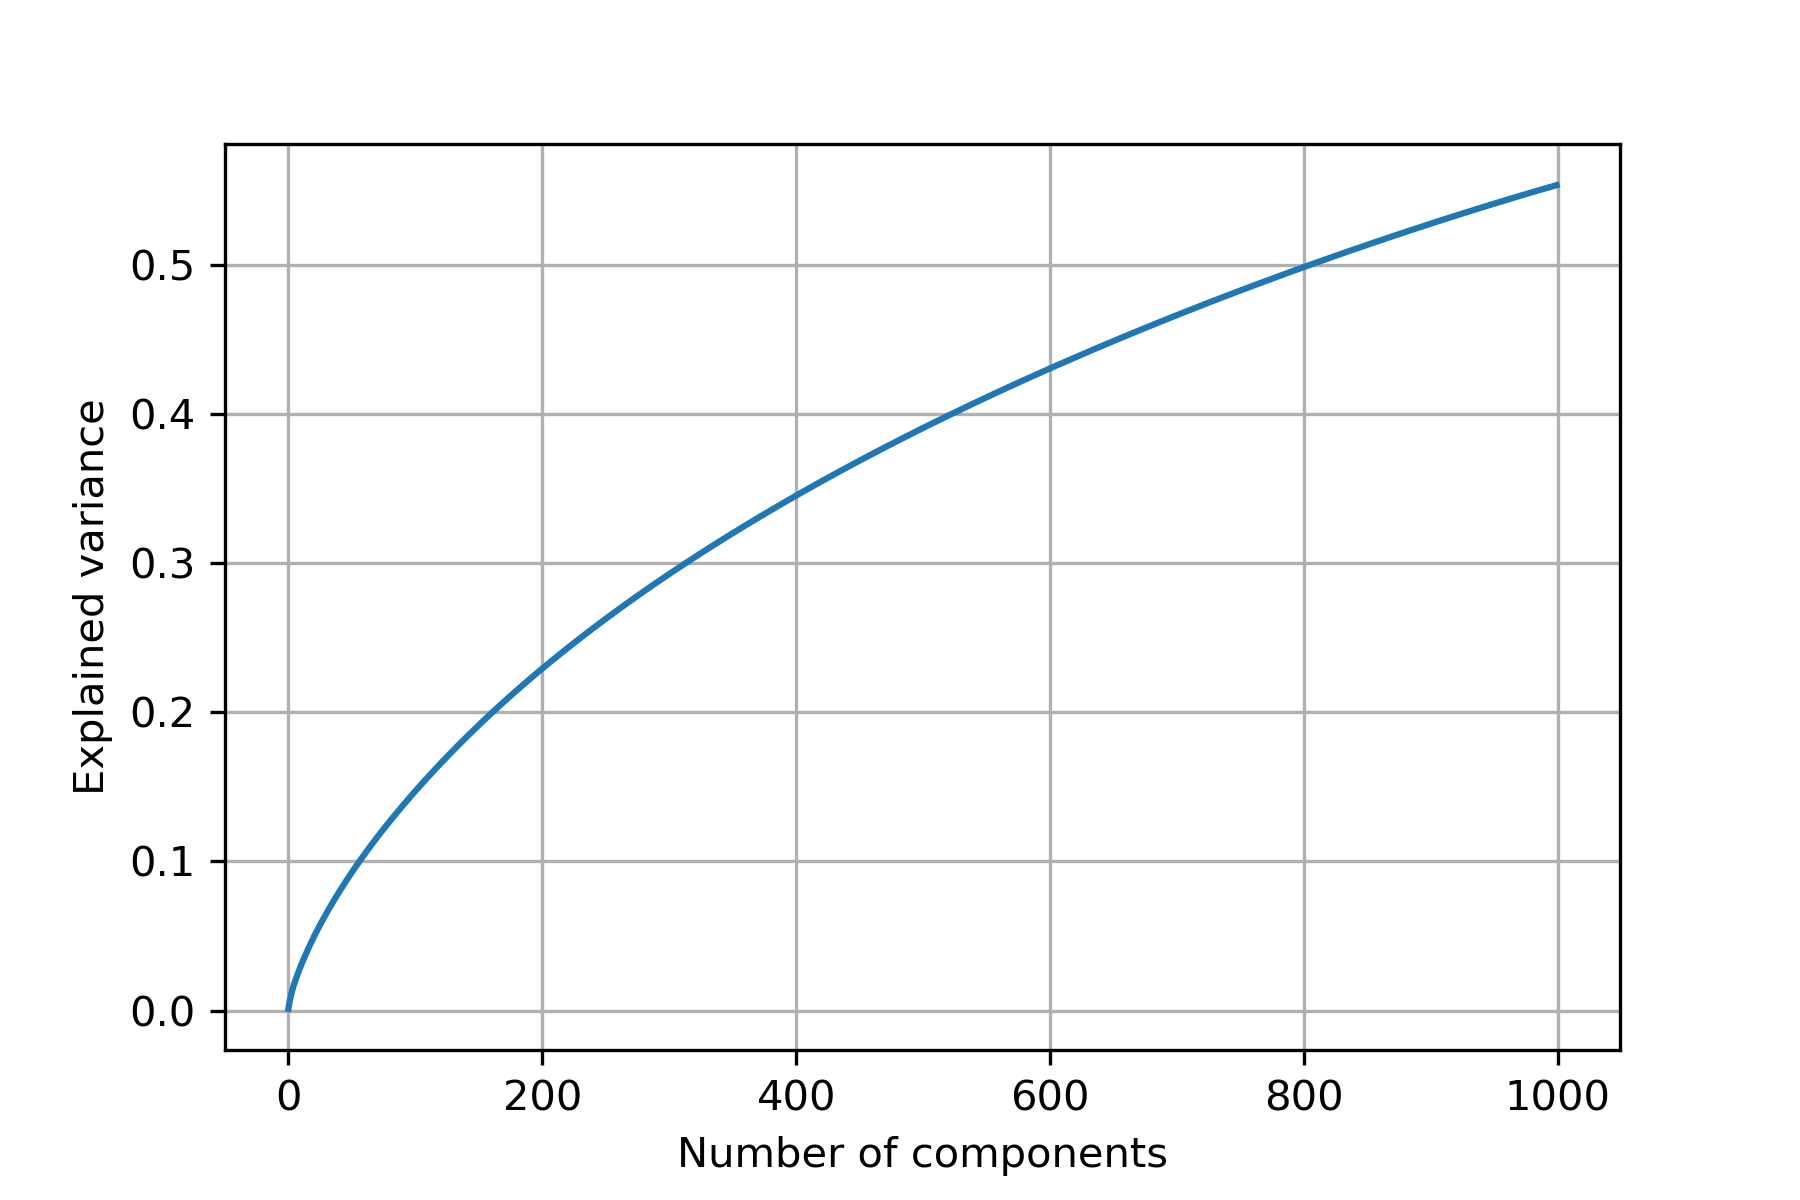
\includegraphics[width=0.6\textwidth]{3-a.png}
	\caption{Cumulative explained variance over number of components involved.}
	\label{fig:explanedVar}
\end{figure}

\begin{figure}[H]
	\centering
	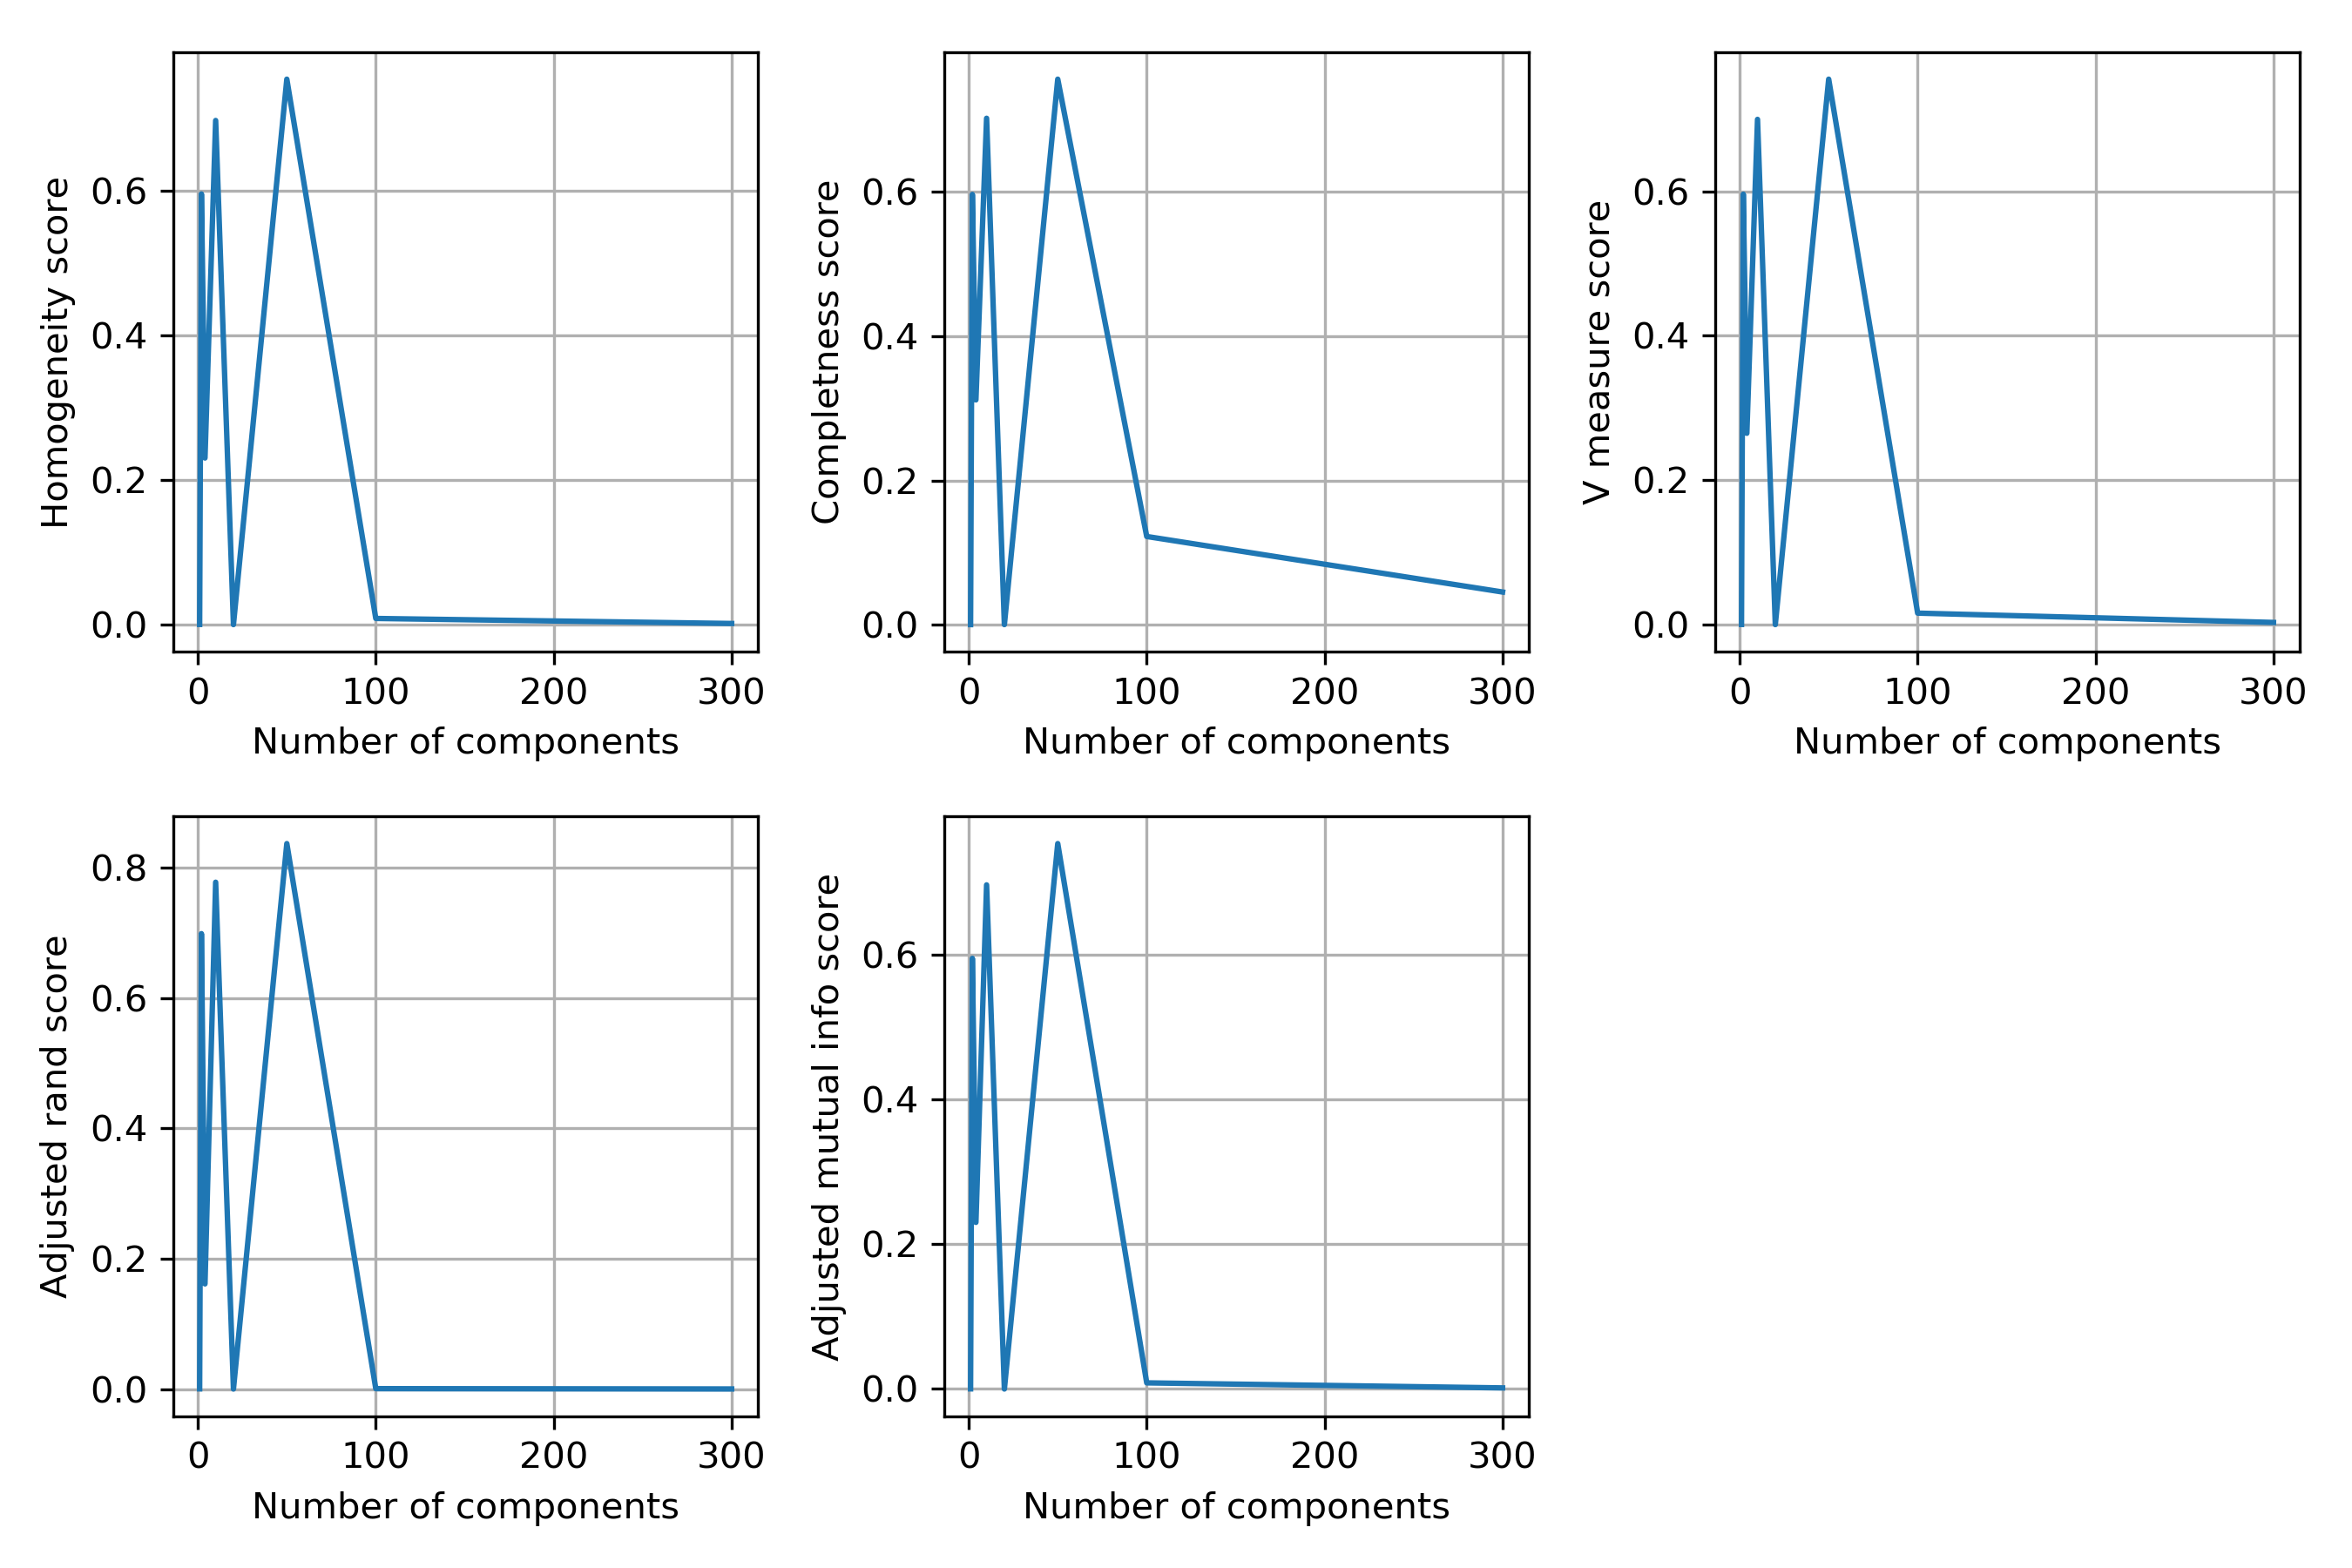
\includegraphics[width=1\textwidth]{3-b-svd-5-measures.png}
	\caption{5 measures using SVD against number of components $r$.}
	\label{fig:svd5}
\end{figure}

\begin{figure}[H]
	\centering
	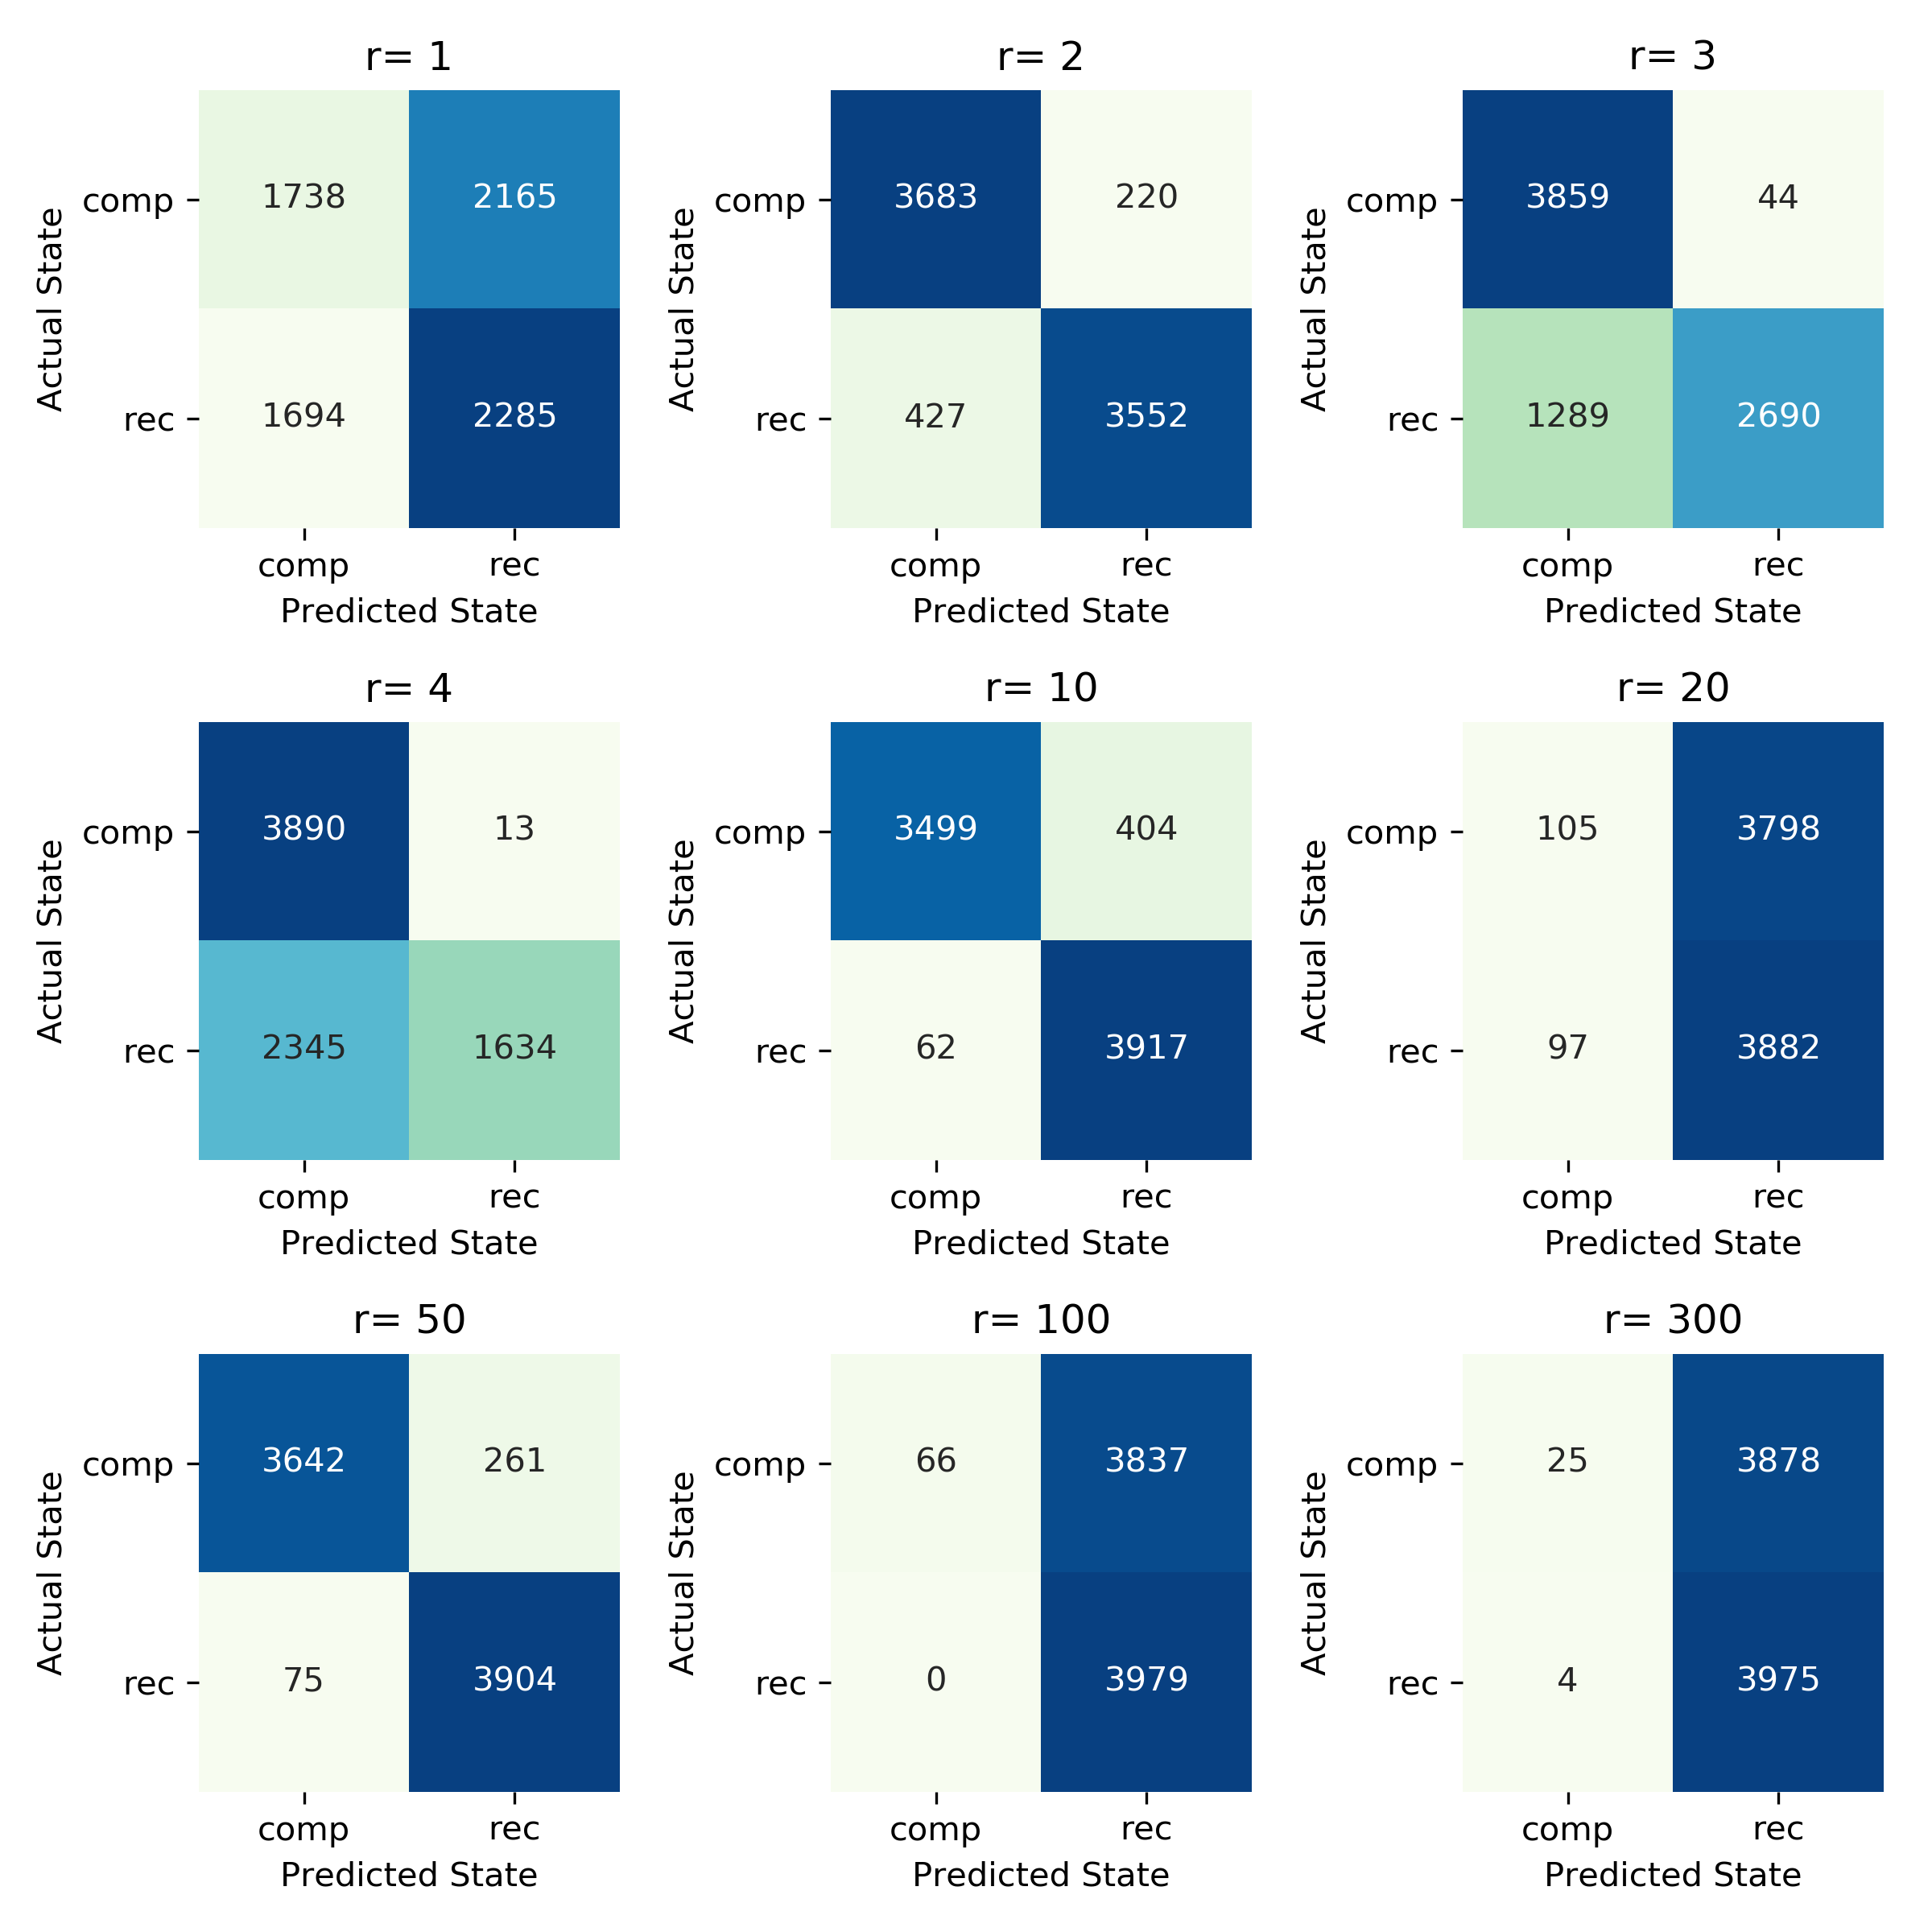
\includegraphics[width=1\textwidth]{3-b-svd-cont-matrix.png}
	\caption{Contingency matrix using SVD with variation on number of components $r$.}
	\label{fig:svdcm}
\end{figure}

\begin{figure}[H]
	\centering
	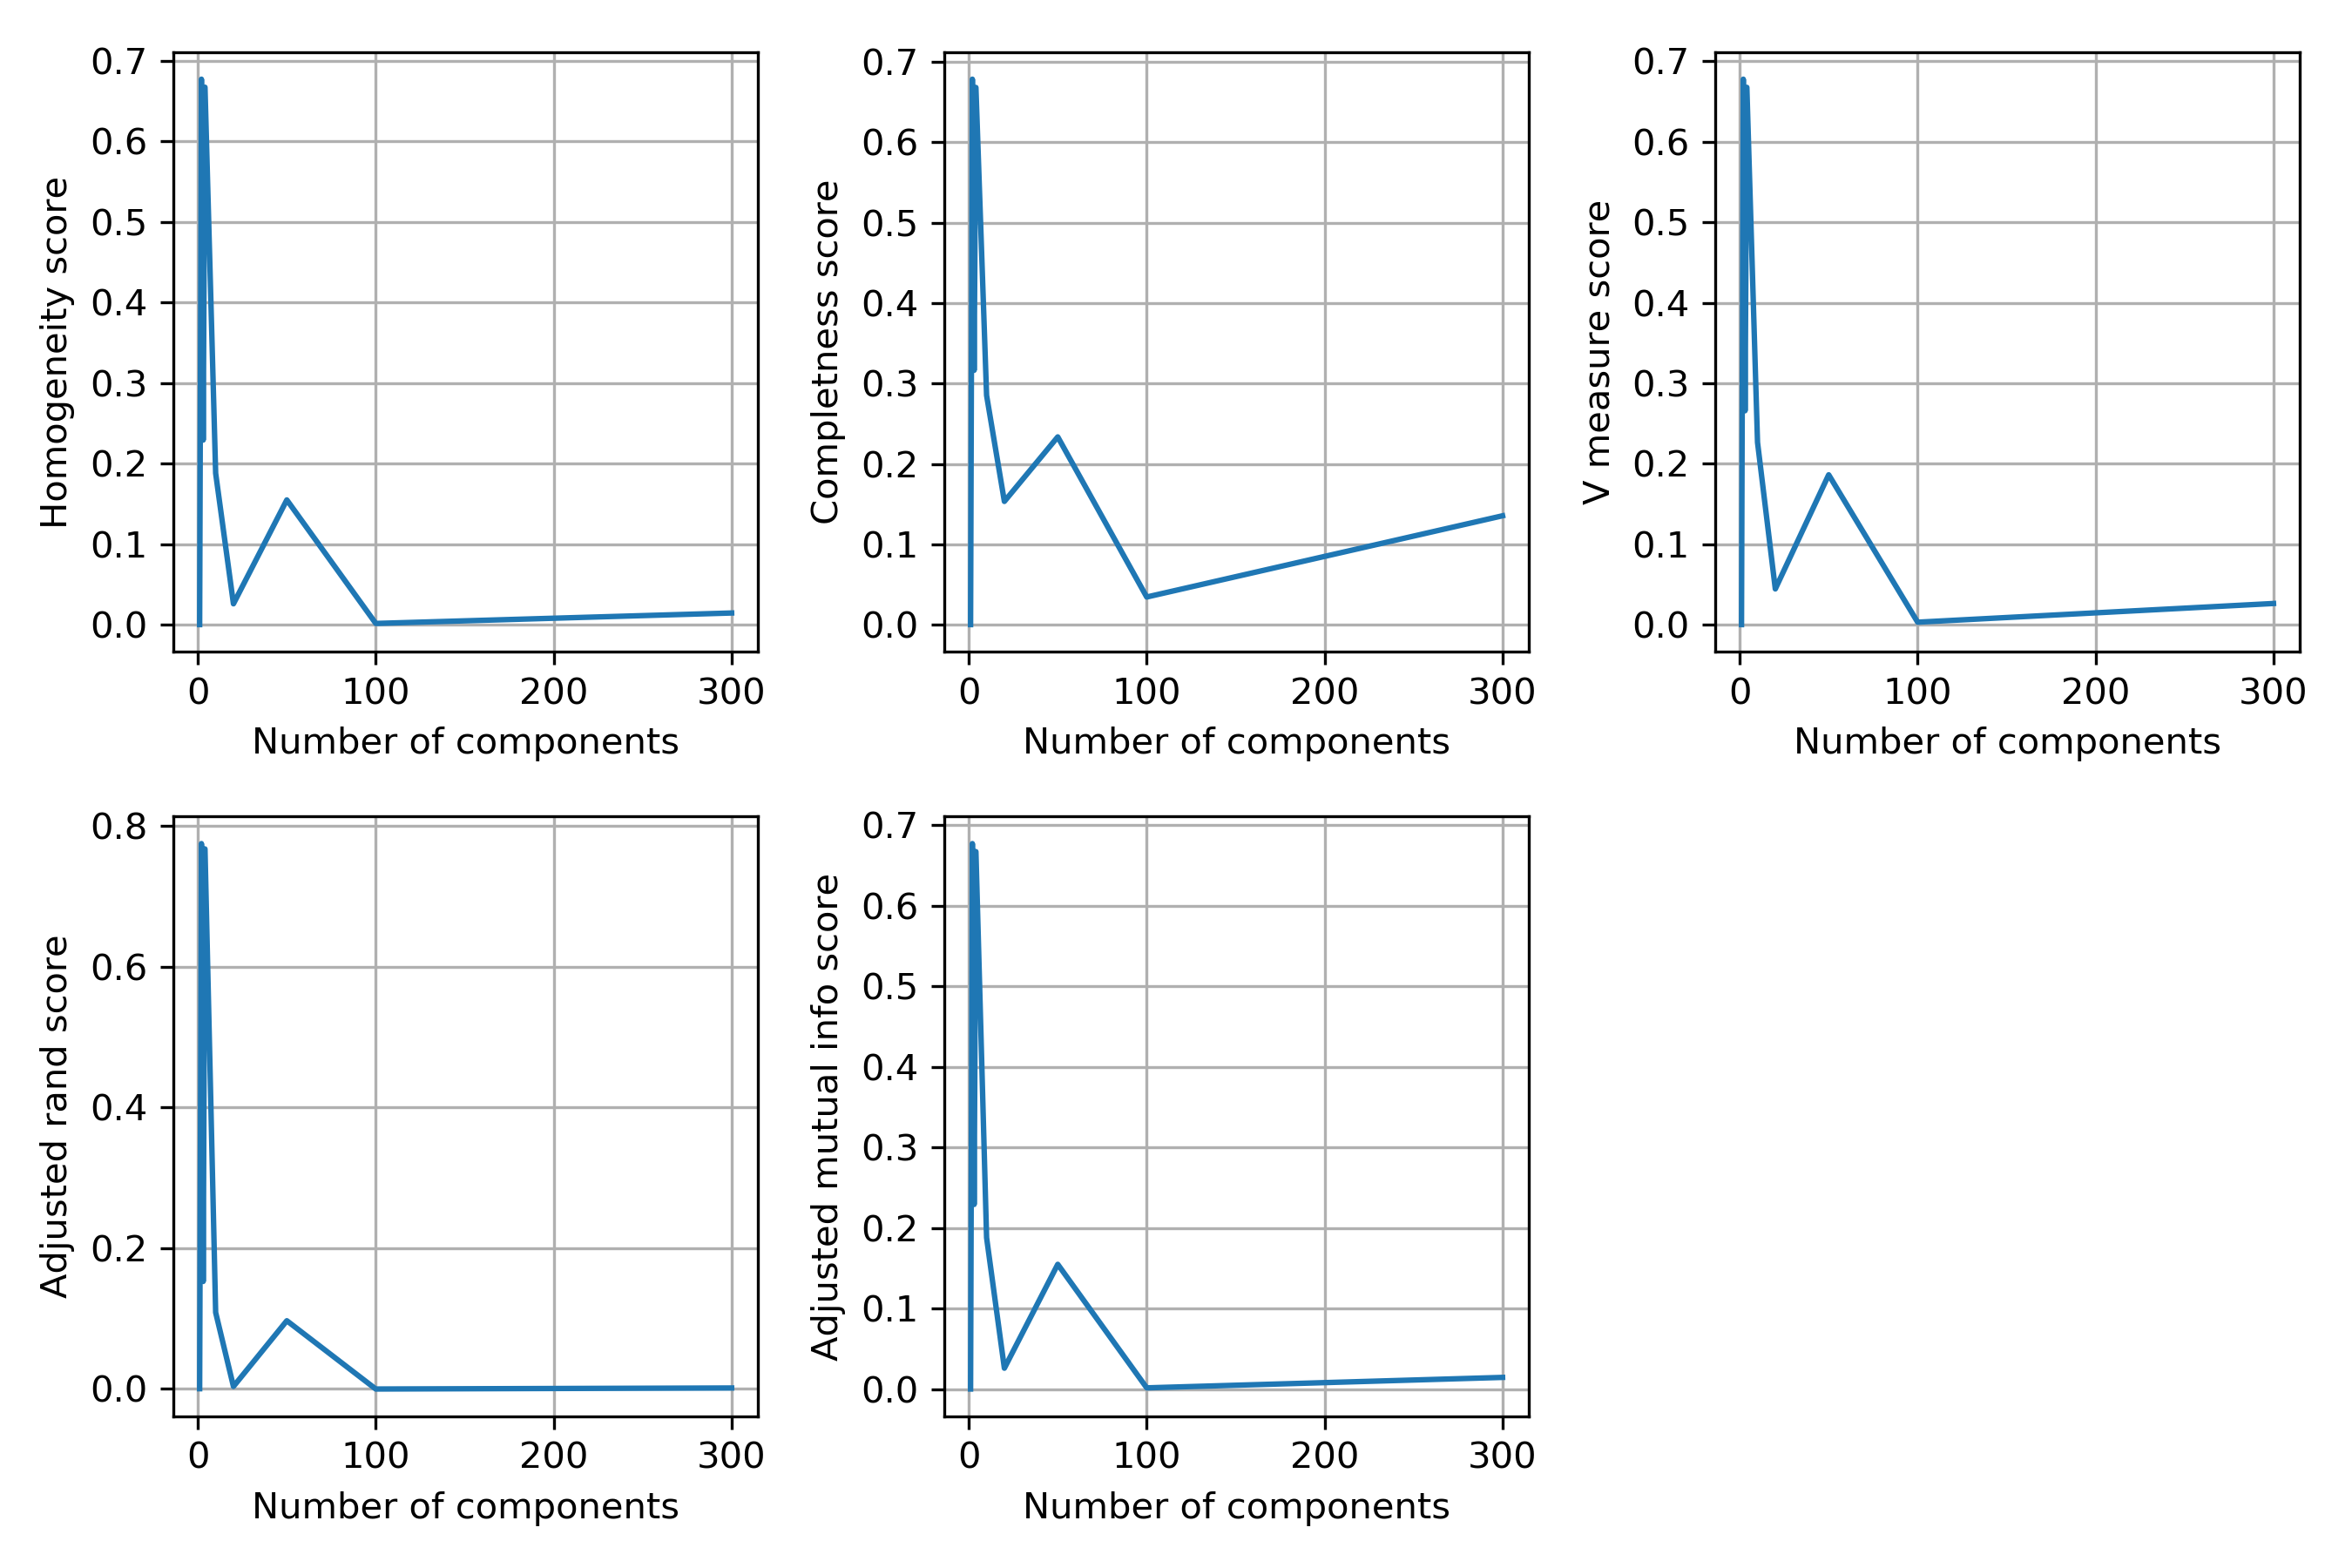
\includegraphics[width=1\textwidth]{3-b-nmf-5-measures.png}
	\caption{5 measures using NMF against number of components $r$. }
	\label{fig:nmf5}
\end{figure}

\begin{figure}[H]
	\centering
	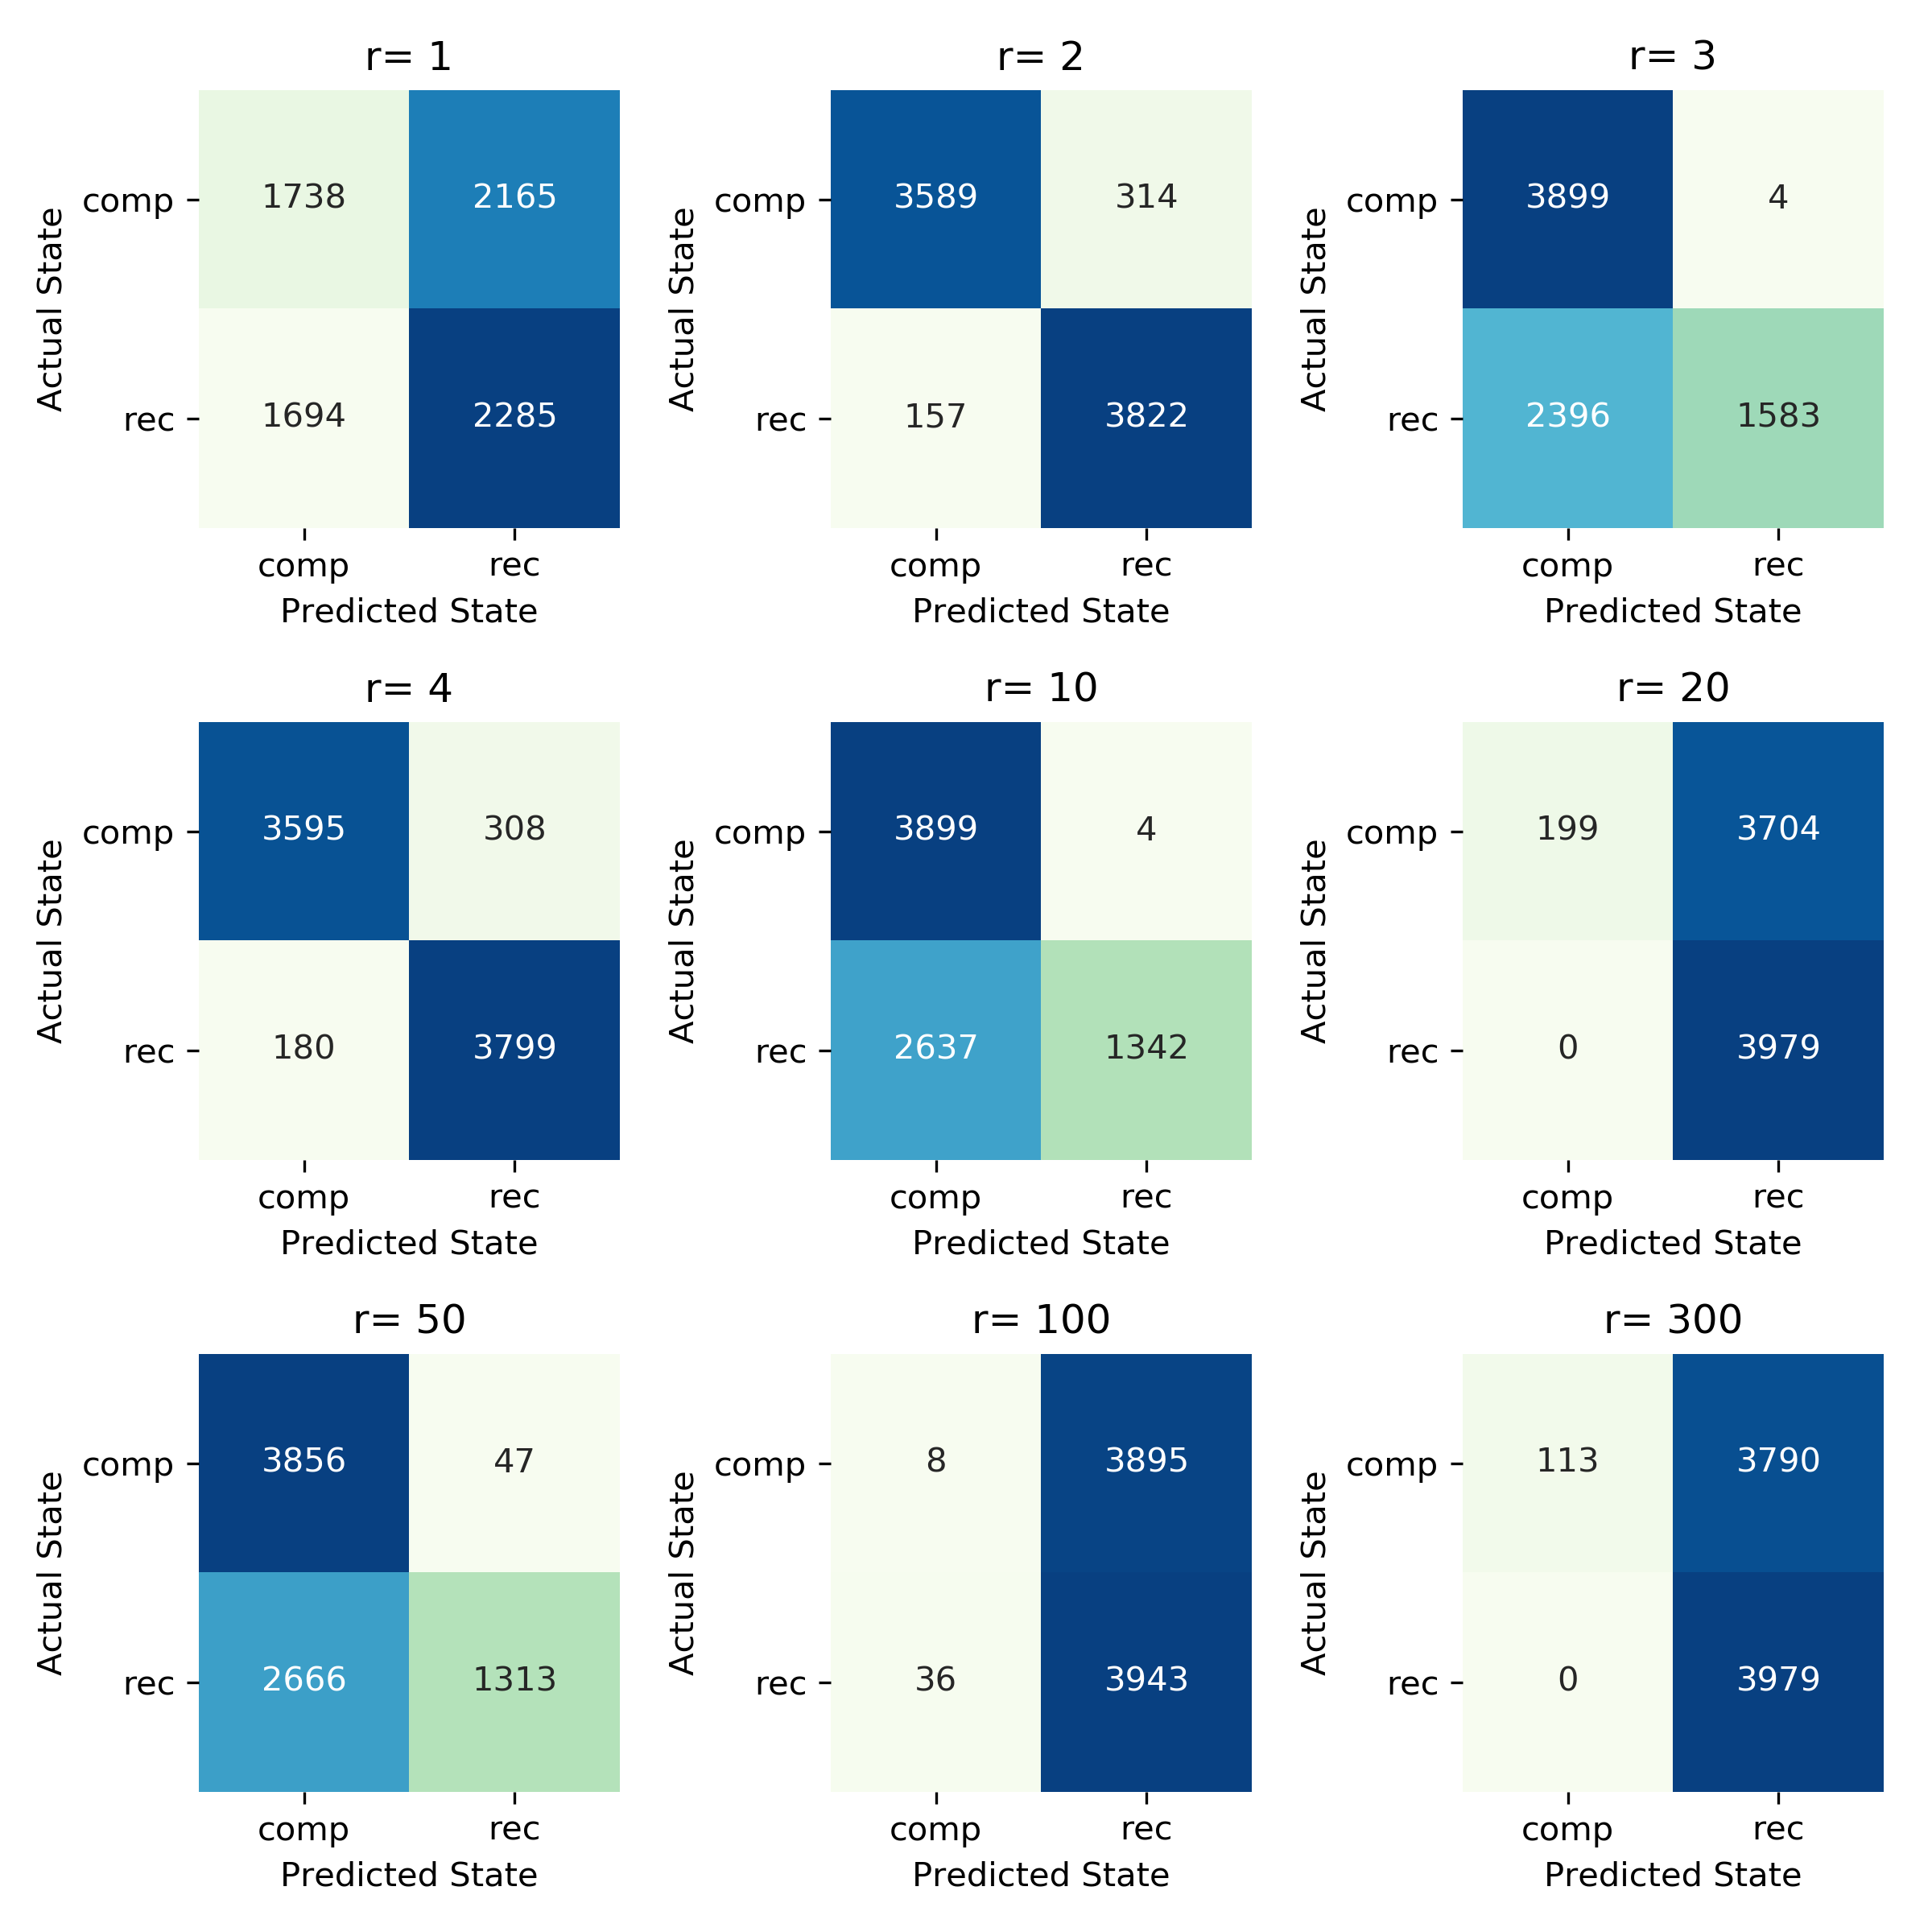
\includegraphics[width=1\textwidth]{3-b-nmf-cont-matrix.png}
	\caption{Contingency matrix using SVD with variation on number of components $r$.}
	\label{fig:nmfcm}
\end{figure}


% ------------------------------------------------------------------------------------------------------------
\paragraph{Question 4} 
\paragraph{} (a) Our best result comes from SVD with $r=50$. Figure \ref{fig:p2d} shows the distribution of observations by projecting the reduced feature matrix into a 2-dimensional space. As we could observe from the figure, the two classes are mostly separated with overlaps. 

\paragraph{} (b)
\begin{itemize}
	\setlength{\itemsep}{0pt}
	\item Figure \ref{fig:p2dunitvar} shows the result if we first perform unit variance scaling. Since the two classes are heavily overlapped, K-means is unable to produce meaningful results.
	\item Figure \ref{fig:p2dlog} shows the distribution of observations with log transformation. As for the general case, log-transformation makes a distribution more "normal" and therefore may have a positive effect on the results. For our case, however, we do not observe an increase, with 5 measures scores close to the unprocessed case. 
	\item Figure \ref{fig:p2dloguv} and \ref{fig:p2duvlog} are the results by applying log transformation and unit variance scaling in different orders. Both of them showed minor improvements to log-transformation-only result. 
\end{itemize}
  

\begin{figure}[H]
	\centering
	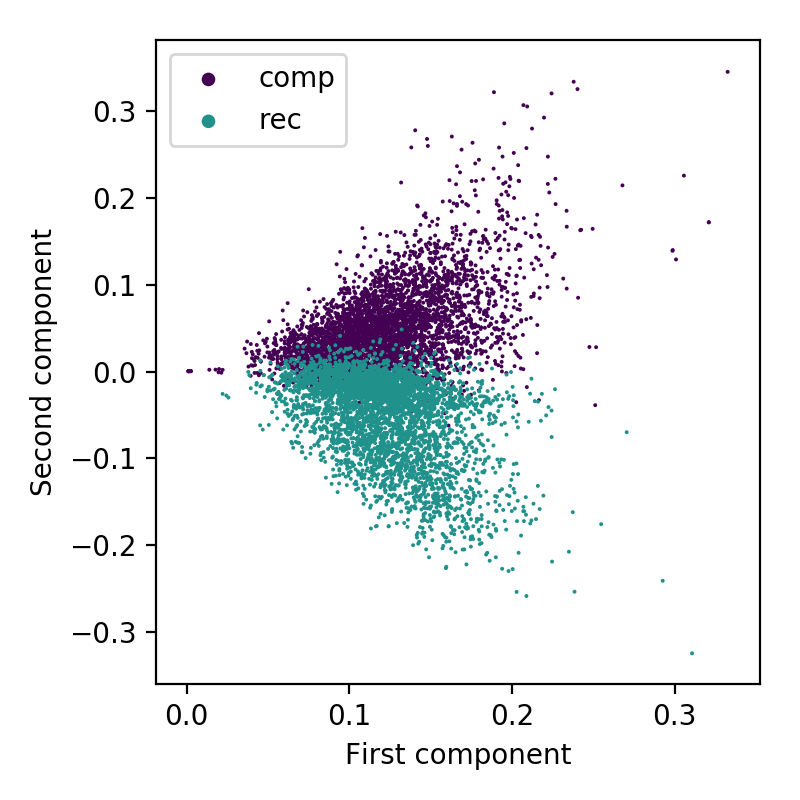
\includegraphics[width=0.5\textwidth]{4-a.png}
	\caption{Distribution of observations using SVD with $r=50$.}
	\label{fig:p2d}
\end{figure}

\begin{figure}[H]
	\centering
	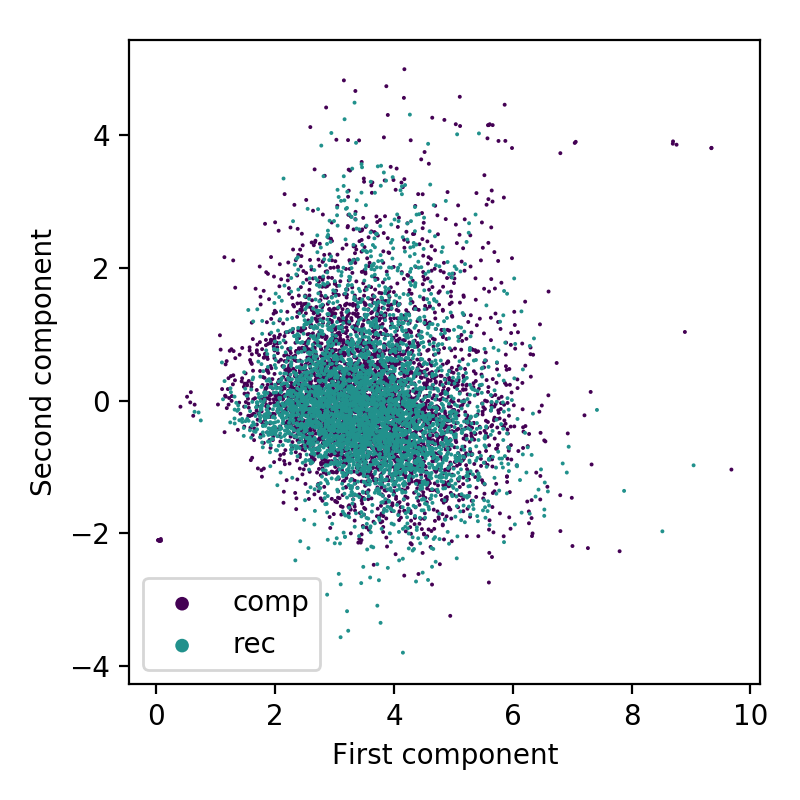
\includegraphics[width=0.5\textwidth]{4-b-unit-var.png}
	\caption{Distribution of observations using SVD with $r=50$ with unit variance scaling.}
	\label{fig:p2dunitvar}
\end{figure}

\begin{figure}[H]
	\centering
	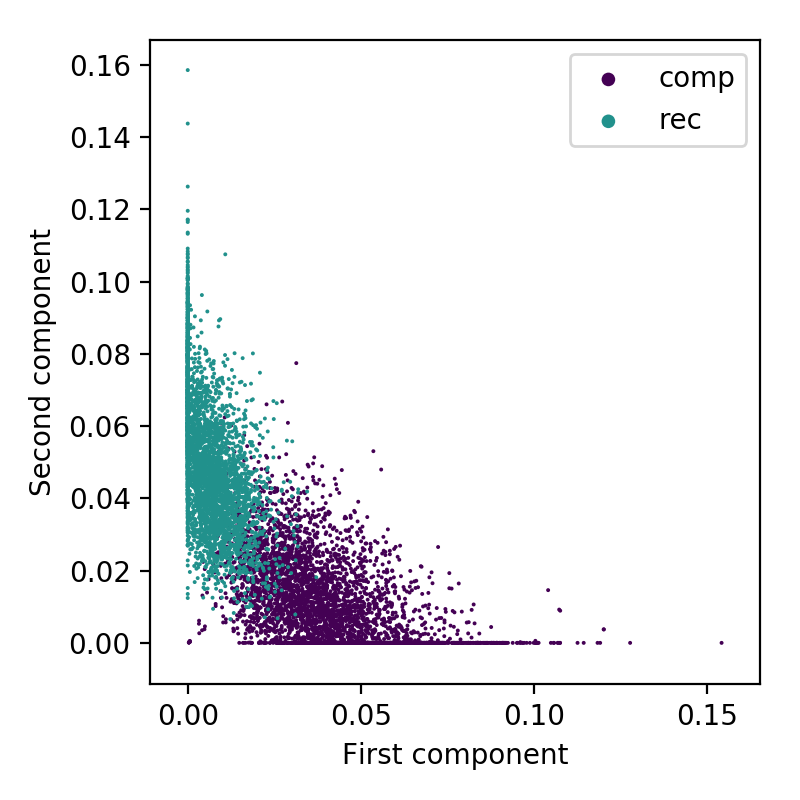
\includegraphics[width=0.5\textwidth]{4-b-log.png}
	\caption{Distribution of observations using SVD with $r=50$ with log transformation.}
	\label{fig:p2dlog}
\end{figure}

\begin{figure}[H]
	\centering
	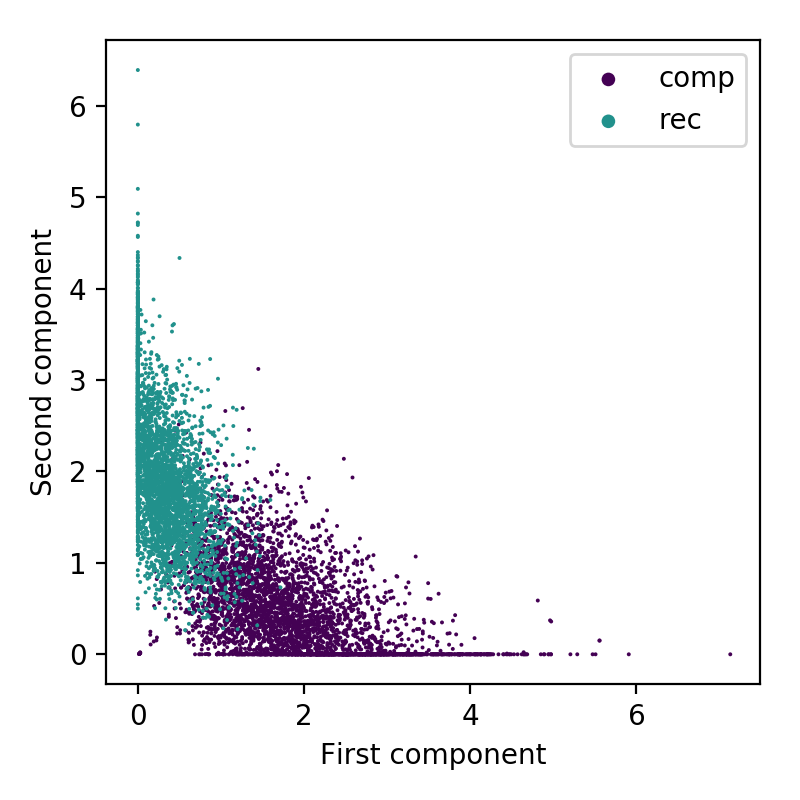
\includegraphics[width=0.5\textwidth]{4-b-log-unit-var.png}
	\caption{Distribution of observations using SVD with $r=50$ with first log transformation followed by unit variance scaling.}
	\label{fig:p2dloguv}
\end{figure}

\begin{figure}[H]
	\centering
	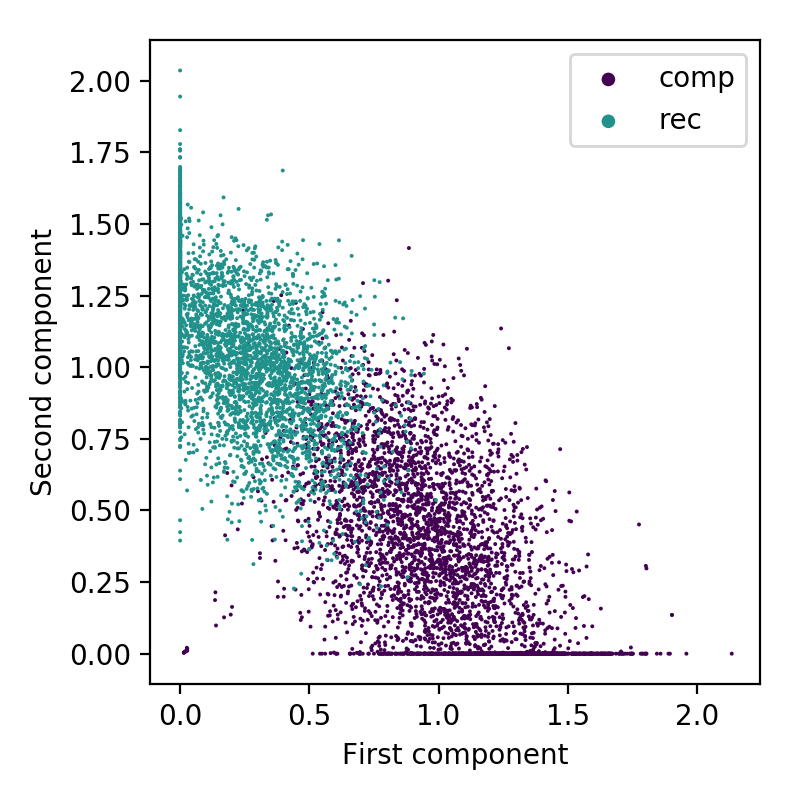
\includegraphics[width=0.5\textwidth]{4-b-unit-var-log.png}
	\caption{Distribution of observations using SVD with $r=50$ with first unit variance scaling followed by log transformation.}
	\label{fig:p2duvlog}
\end{figure}
% ------------ ------------------------------------------------------------------------------------------------
\paragraph{Question 5}
Our best result comes from NMF with $r=20$. Figure \ref{fig:5p2d} shows the by projecting the reduced feature matrix into a 2-dimensional space. The results are listed as follows.
\begin{itemize}
	\setlength{\itemsep}{0pt}
	\item Figure \ref{fig:5p2dunitvar} shows the result if we first perform unit variance scaling. 
	\item Figure \ref{fig:5p2dlog} shows the distribution of observations with log transformation.
	\item Figure \ref{fig:5p2dloguv} and \ref{fig:5p2duvlog} are the results by applying log transformation and unit variance scaling in different orders.
\end{itemize}
As we can see from all 5 figures, all 20 classes are sitting on top of each other, resulting that there is little K-means can do.

\begin{figure}[H]
	\centering
	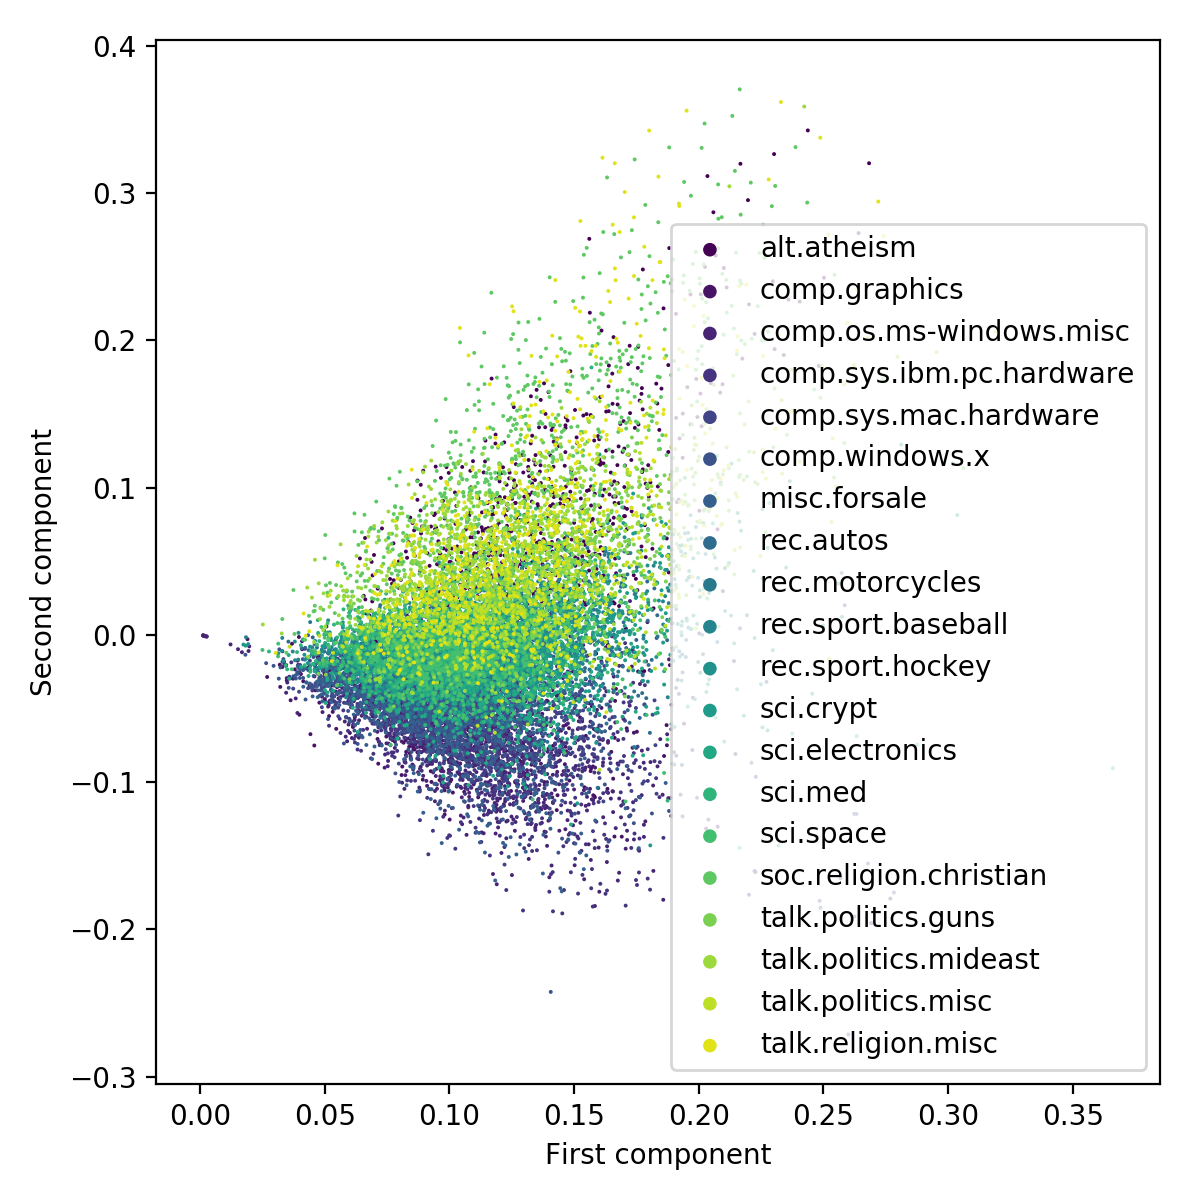
\includegraphics[width=0.5\textwidth]{5-2d-raw.png}
	\caption{Distribution of observations using NMF with $r=20$.}
	\label{fig:5p2d}
\end{figure}

\begin{figure}[H]
	\centering
	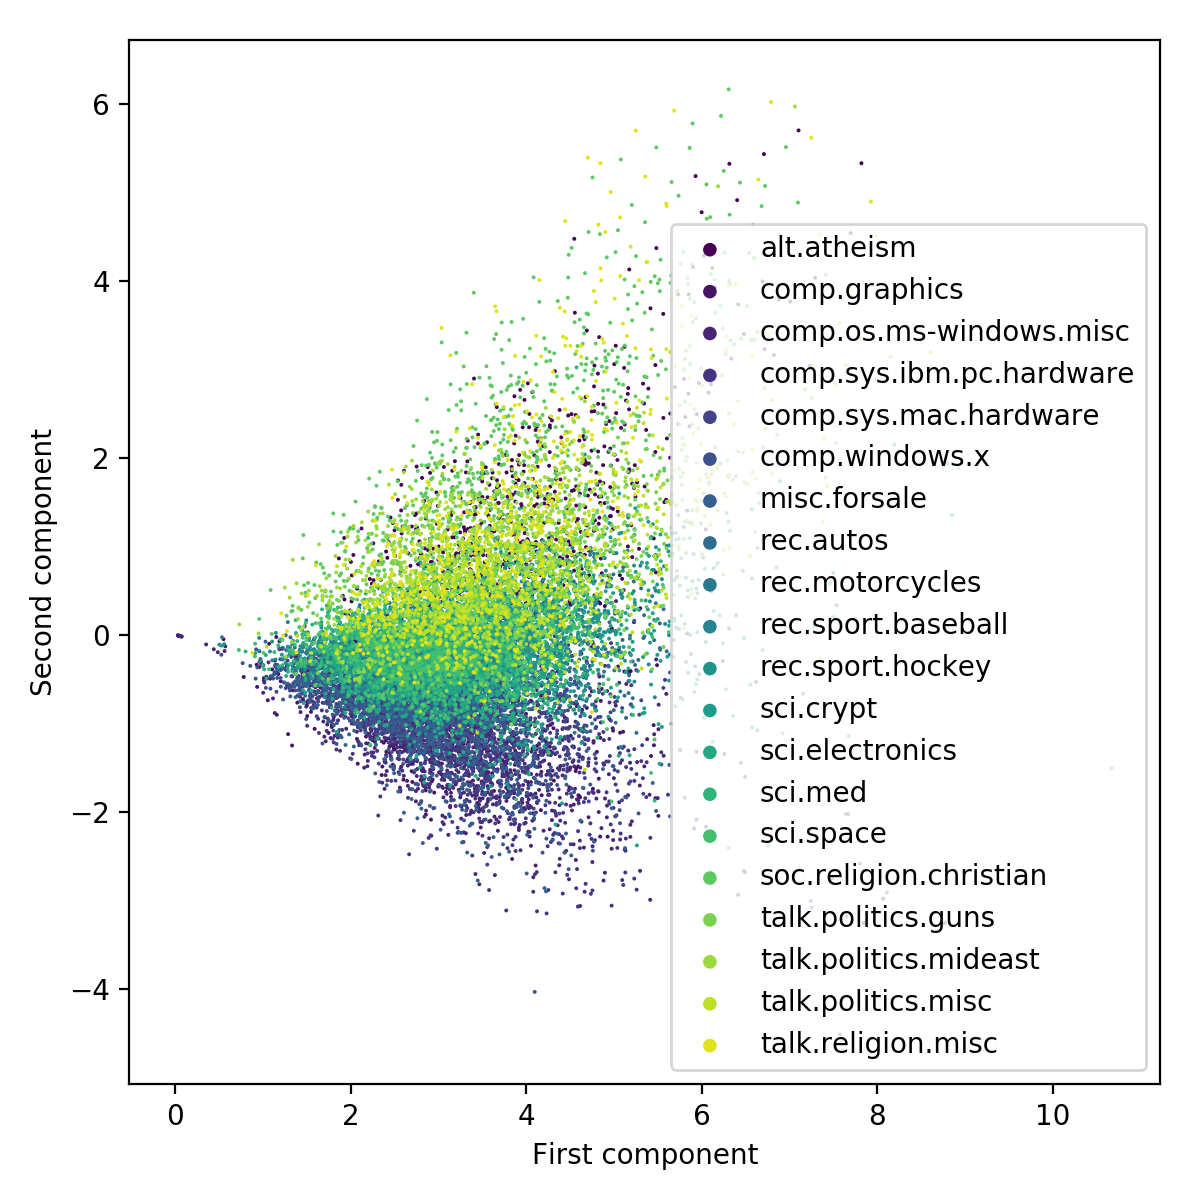
\includegraphics[width=0.5\textwidth]{5-2d-unit-var.png}
	\caption{Distribution of observations using NMF with $r=20$ with unit variance scaling.}
	\label{fig:5p2dunitvar}
\end{figure}

\begin{figure}[H]
	\centering
	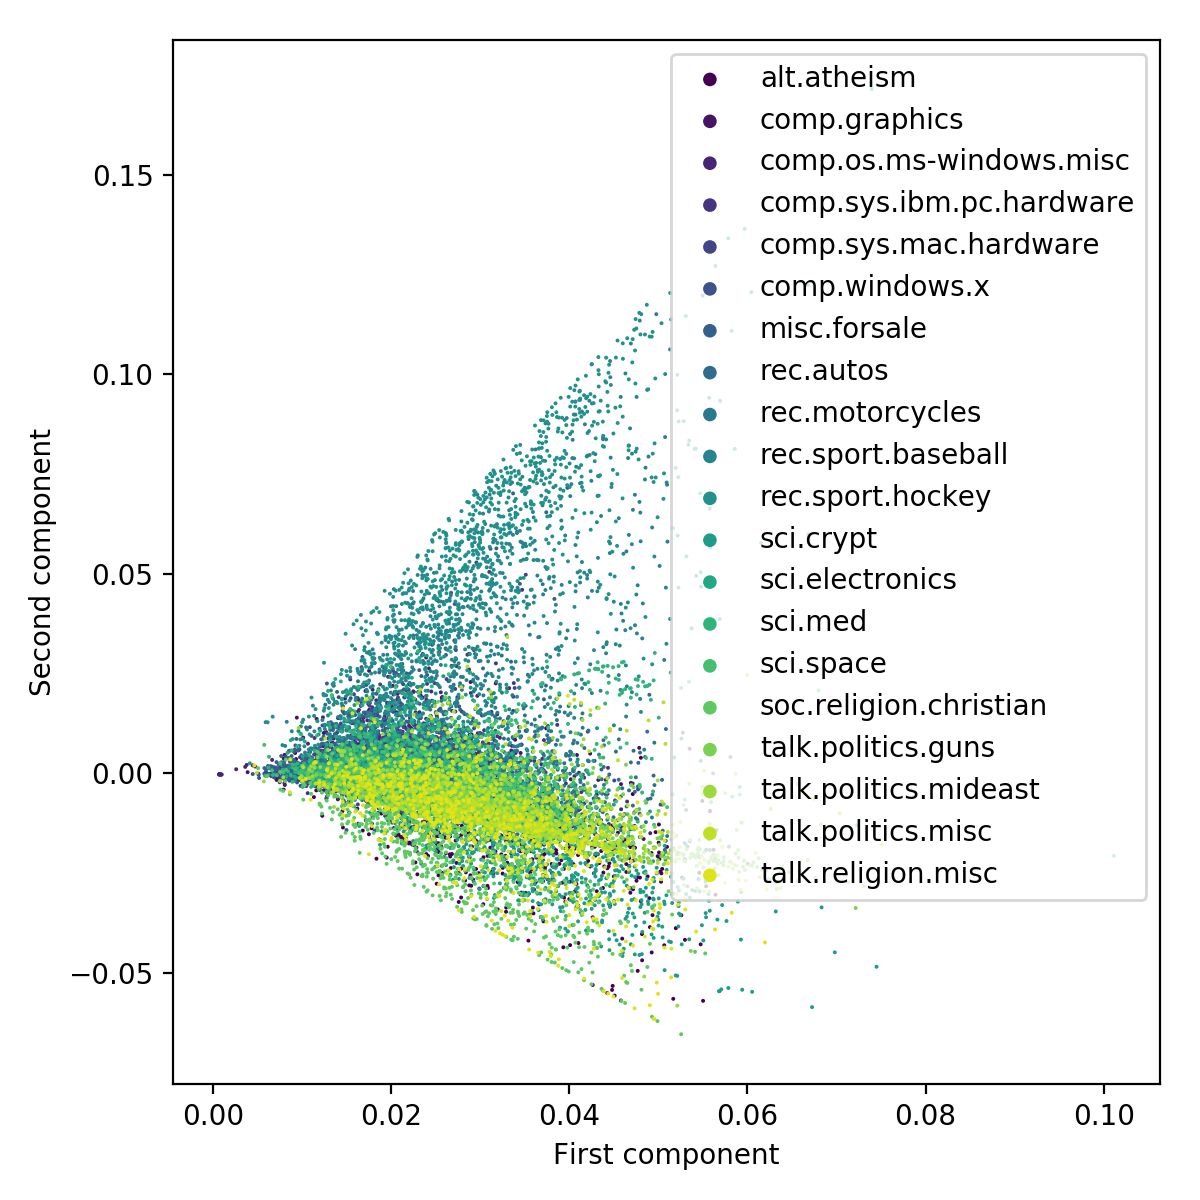
\includegraphics[width=0.5\textwidth]{5-2d-log-transform.png}
	\caption{Distribution of observations using NMF with $r=20$ with log transformation.}
	\label{fig:5p2dlog}
\end{figure}

\begin{figure}[H]
	\centering
	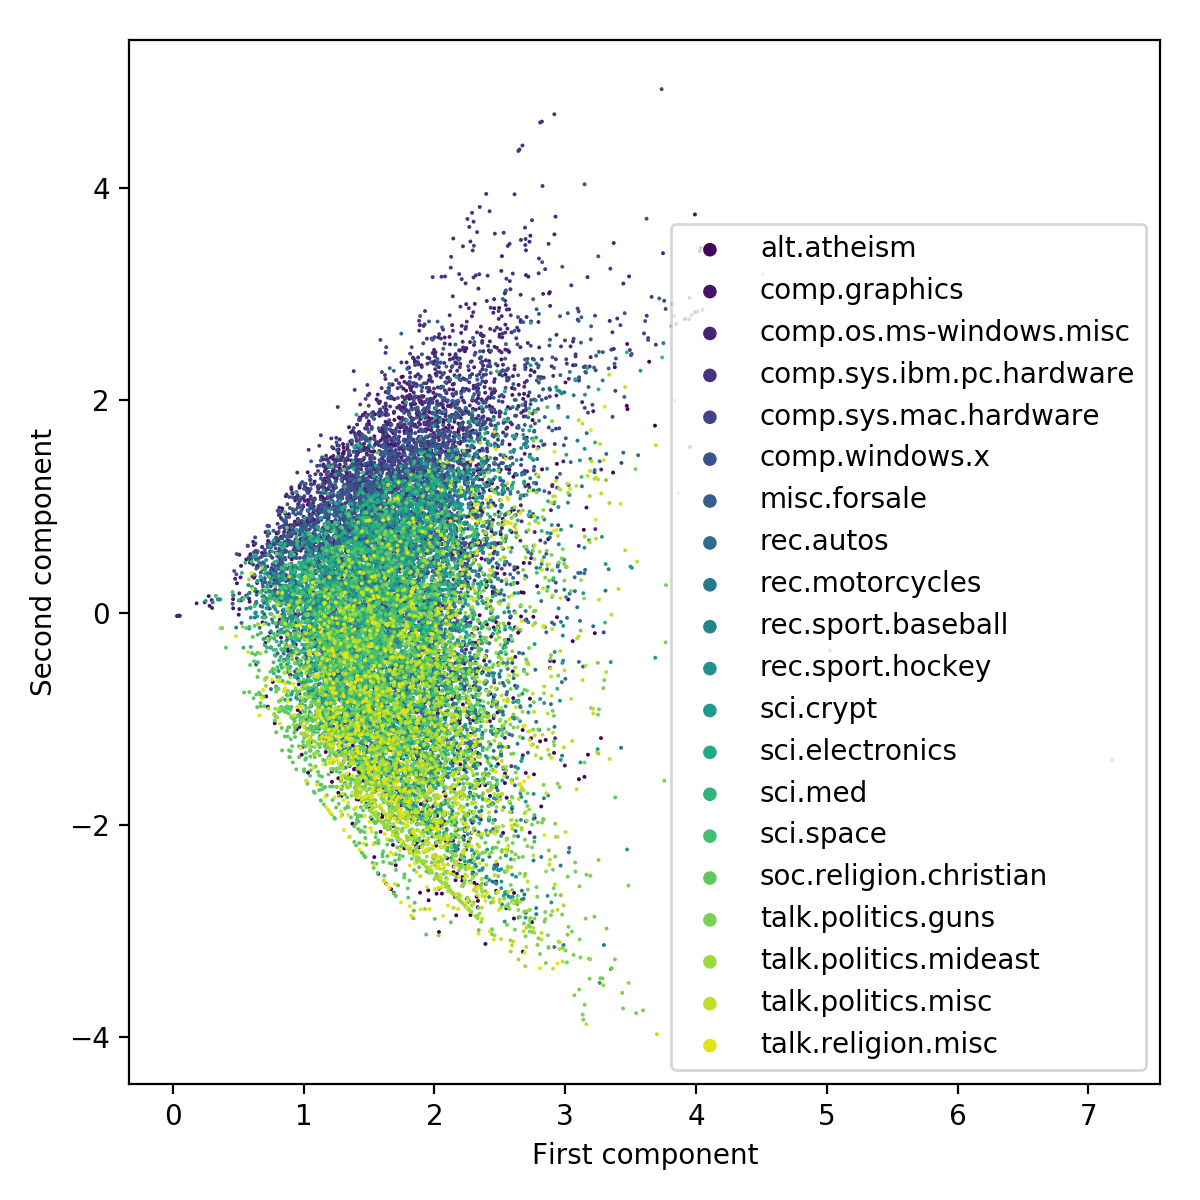
\includegraphics[width=0.5\textwidth]{5-2d-log-unit-var.png}
	\caption{Distribution of observations using NMF with $r=20$ with first log transformation followed by unit variance scaling.}
	\label{fig:5p2dloguv}
\end{figure}

\begin{figure}[H]
	\centering
	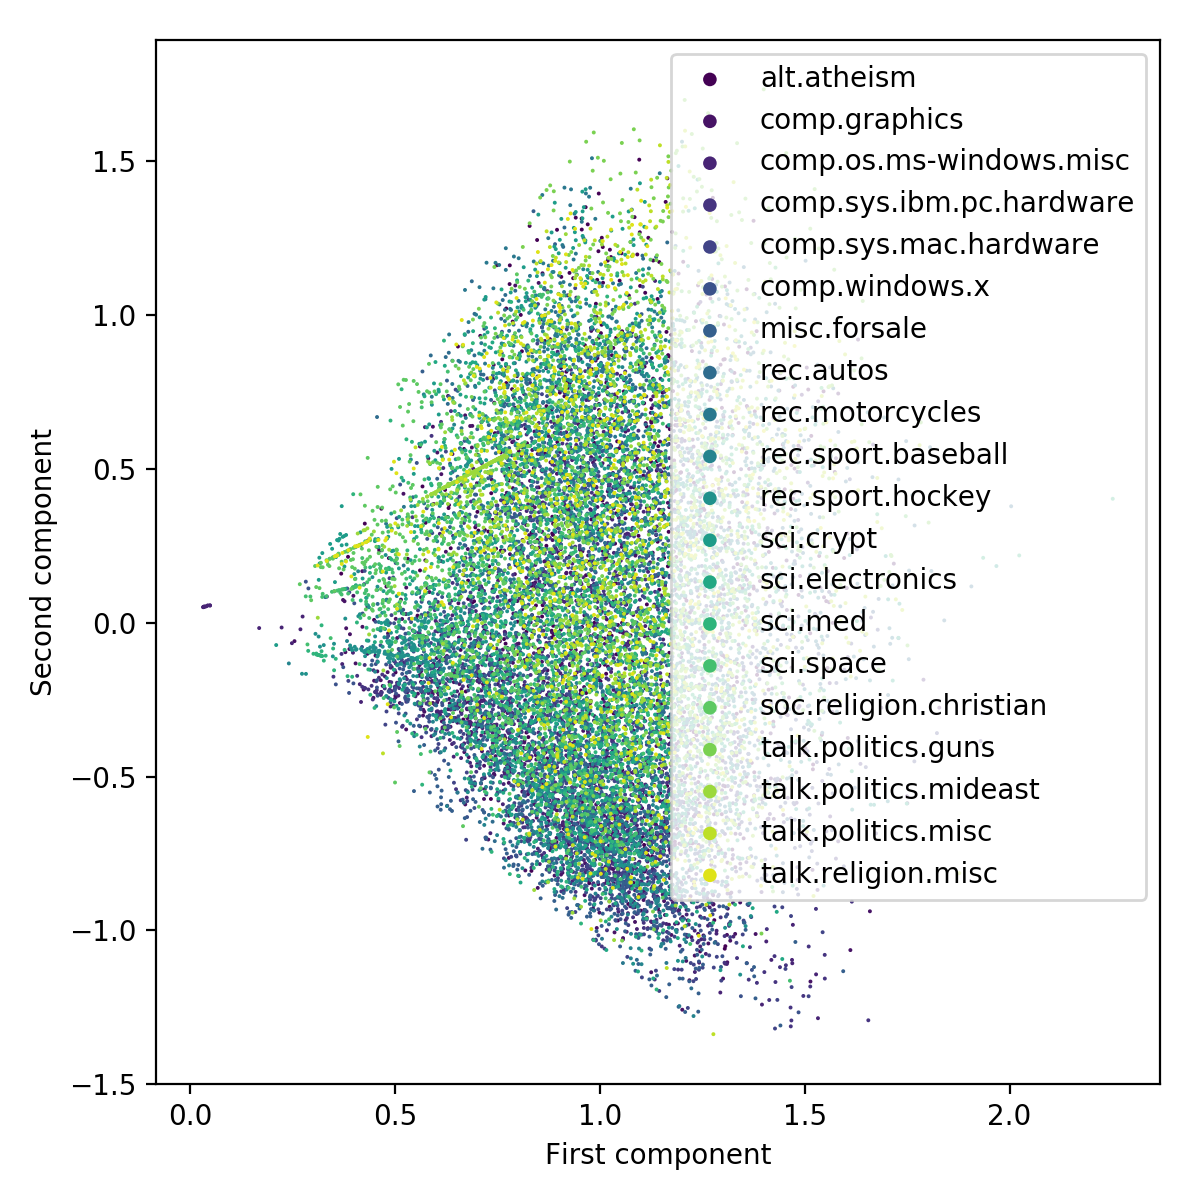
\includegraphics[width=0.5\textwidth]{5-2d-unit-var-log.png}
	\caption{Distribution of observations using NMF with $r=20$ with first unit variance scaling followed by log transformation.}
	\label{fig:5p2duvlog}
\end{figure}

\end{document}	